\chapter{Lecture 8 - Manuel Araújo}

\section{Feynman Integrals in Finite Dimensions}

Our study will involve integrals of the form
\begin{equation*}
  \int_{\Rbb^n} \drm^n x \euler^{-Q(x, x)} = \frac{\pi^{\frac{n}{2}}}{\sqrt{\det Q}}
\end{equation*}
for a nondegenerate quadratic form $Q$.

\subsection{Expectation value of monomials}

We are interested in expectation values
\begin{equation*}
  \avg{x_{i_1} \dots x_{i_{2m}}}
  = \frac{
    \int_{\Rbb^n} \drm^n x \euler^{-\frac{1}{2}Q(x, x)} x_{i_1} \dots x_{i_{2m}}
  }{
    \int_{\Rbb^n} \drm^n x \euler^{-\frac{1}{2}Q(x, x)}
  }.
\end{equation*}
To compute these consider
\begin{equation*}
  W(J) = \int_{\Rbb^n} \drm^n x \euler^{-\frac{1}{2} Q(x, x) + \langle J, x \rangle}
\end{equation*}
which is such that
\begin{equation*}
  \avg{x_{i_1} \dots x_{i_{2m}}}
  = \frac{\partial}{\partial J_{i_1}} \dots \frac{\partial}{\partial J_{i_{2m}}} \bigg|_{J = 0}.
  \frac{W(J)}{W(0)}
\end{equation*}
Completing the square we get
\begin{align*}
  W(J) 
  &= \euler^{\frac{1}{2} \langle J, Q^{-1} J \rangle}
  \int_{\Rbb^n} \drm^n x
  \euler^{-\frac{1}{2} Q(x, x) + \langle J, x \rangle - \frac{1}{2} \langle J, Q^{-1} x \rangle} \\
  &= \euler^{\frac{1}{2} \langle J, Q^{-1} J \rangle}
  \int_{\Rbb^n} \drm^n x
  \euler^{- \frac{1}{2} Q (x - Q^{-1} J, x - Q^{-1} J) } \\
  &= \euler^{\frac{1}{2} \langle J, Q^{-1} J \rangle}
  \underbrace{\int_{\Rbb^n} \drm^n y \euler^{- \frac{1}{2} Q (y, y) }}_{W(0)}
\end{align*}
therefore
 \begin{equation*}
  \avg{x_{i_1} \dots x_{i_{2m}}}
  = \frac{\partial}{\partial J_{i_1}} \dots \frac{\partial}{\partial J_{i_{2m}}} \bigg|_{J = 0}
  \euler^{-\frac{1}{2} \langle J, Q^{-1} J \rangle}
\end{equation*}
and Taylor expanding the exponential we obtain
\begin{align*}
  \avg{x_{i_1} \dots x_{i_{2m}}}
  &= \frac{\partial}{\partial J_{i_1}} \dots \frac{\partial}{\partial J_{i_{2m}}} \bigg|_{J = 0}
  \sum_{p = 0}^\infty \frac{1}{2^p p!}
  \biggl( \sum_{j, k} J_j J_k Q_{jk}^{-1} \biggr)^p \\
  &= \frac{1}{2^m m!} \frac{\partial}{\partial J_{i_1}} \dots \frac{\partial}{\partial J_{i_{2m}}} \bigg|_{J = 0}
  \biggl( \sum_{j, k} J_j J_k Q_{jk}^{-1} \biggr)^m \\
  &= \frac{1}{2^m m!} \sum_{\sigma \in S_{2m}} Q_{i_{\sigma_1} i_{\sigma_2}}^{-1} \dots
  Q_{i_{\sigma_{2m-1}} i_{\sigma_{2m}}}^{-1}.
\end{align*}
We can exploit the symmetry of this formula by noticing that there exists a free action of the group
\begin{equation*}
  S_m \ltimes \Zbb_2^m
\end{equation*}
corresponding to permutations of the elements in each pair, as well as the order of the pairings. We call the equivalence classes of permutations corresponding to picking (unordered) pairs of elements by pairings, and write the corresponding quotient group
\begin{equation*}
  \text{Matchings}_{2m} = \bigslant{S_{2m}}{S_m \ltimes \Zbb_2^m}.
\end{equation*}
The size of any orbit is $| \Ocal (\sigma) | = 2^m m!$ so we sum on matchings to obtain
\begin{align*}
  \avg{x_{i_1} \dots x_{i_{2m}}}
  &= \sum_{[\sigma]}
  Q_{i_{\sigma_1} i_{\sigma_2}}^{-1} \dots Q_{i_{\sigma_{2m-1}} i_{\sigma_{2m}}}^{-1} \\
  &= \sum_{[\sigma]} (Q^{-1})^{\otimes m} \circ \sigma \circ \bigl(x_{i_1} \otimes \dots \otimes x_{i_{2m}}\bigr).
\end{align*}

\begin{example}
  Consider a monomial $\psi = x_1 x_2 x_3 x_4$, then
  \begin{align*}
    \avg{x_1 x_2 x_3 x_4}
    &= 
    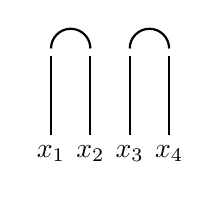
\begin{tikzpicture}[scale=.5, baseline=4mm]
      % lines
      \draw[thick] (0, 0) node[anchor=north] {$x_1$} -- (0, 2);
      \draw[thick] (1, 0) node[anchor=north] {$x_2$}-- (1, 2);
      \draw[thick] (2, 0) node[anchor=north] {$x_3$} -- (2, 2);
      \draw[thick] (3, 0) node[anchor=north] {$x_4$} -- (3, 2);
      % pairings
      \draw[thick] (0, 2.2) arc (180:0:.5);
      \draw[thick] (2, 2.2) arc (180:0:.5);
    \end{tikzpicture}
    +
    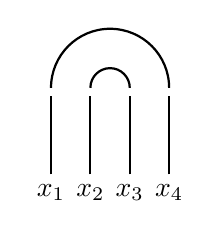
\begin{tikzpicture}[scale=.5, baseline=4mm]
      % lines
      \draw[thick] (0, 0) node[anchor=north] {$x_1$} -- (0, 2);
      \draw[thick] (1, 0) node[anchor=north] {$x_2$}-- (1, 2);
      \draw[thick] (2, 0) node[anchor=north] {$x_3$} -- (2, 2);
      \draw[thick] (3, 0) node[anchor=north] {$x_4$} -- (3, 2);
      % pairings
      \draw[thick] (0, 2.2) arc (180:0:1.5);
      \draw[thick] (1, 2.2) arc (180:0:.5);
    \end{tikzpicture}
    +
    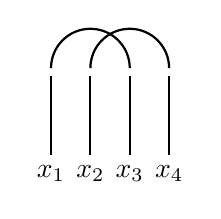
\begin{tikzpicture}[scale=.5, baseline=4mm]
      % lines
      \draw[thick] (0, 0) node[anchor=north] {$x_1$} -- (0, 2);
      \draw[thick] (1, 0) node[anchor=north] {$x_2$}-- (1, 2);
      \draw[thick] (2, 0) node[anchor=north] {$x_3$} -- (2, 2);
      \draw[thick] (3, 0) node[anchor=north] {$x_4$} -- (3, 2);
      % pairings
      \draw[thick] (0, 2.2) arc (180:0:1);
      \draw[thick] (1, 2.2) arc (180:0:1);
    \end{tikzpicture} \\
    &= Q_{12}^{-1} Q_{34}^{-1} + Q_{14}^{-1} Q_{23}^{-1} + Q_{13}^{-1} Q_{24}^{-1}.
  \end{align*}
  On the other hand, for the monomial $\psi = x^4$ there is further symmetry, so we get
  \begin{equation*}
    \avg{x^4} = 3 Q_{11}^{-1} Q_{11}^{-1}.
  \end{equation*}
\end{example}

For a general finite-dimensional vector space $V$ the expectation value corresponds to a map
\begin{equation*}
  \avg{\cdot} \colon \Trm V^\vee \longrightarrow \Rbb
\end{equation*}
where $\Trm V^\vee$ denotes the tensor algebra of $V$. Picking a top form $\mu$ on $V$ we can write
\begin{align*}
  \avg{\phi_{i_1} \otimes \dots \otimes \phi_{i_{2m}}}
  &= \frac{
    \int_V \mu \euler^{-\frac{1}{2} Q(x, x)} \phi_{i_1}(x) \dots \phi_{i_{2m}}(x)
  }{
    \int_V \mu \euler^{-\frac{1}{2} Q(x, x)}
  } \\
  &= \sum_{[\sigma]} (Q^{-1})^{\otimes m} \circ \sigma \circ (\phi_{i_1} \otimes \dots \otimes \phi_{i_{2m}})
\end{align*}

The graphical representation systematize the computations. In this context, a \textbf{graph} consists of:
\begin{enumerate}[i)]
  \item a finite set $V$ of \textbf{vertices};
  \item a finite set $HE$ of \textbf{half-edges} (an even number of them);
  \item an \textbf{incidence} map $i: HE \to V$;
  \item a \textbf{matching} $\sigma$ on $HE$.
\end{enumerate}
A graph automorphism permutes vertices and half-edges, respecting $i$ and $\sigma$.

\begin{example}
  The following graph has a nontrivial automorphism
  \begin{equation*}
    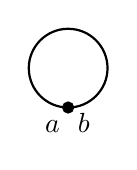
\begin{tikzpicture}
      \draw[fill=black] (0, 0) circle (2pt);
      \draw[thick] (0, .5) circle (5mm);
      \node at (-.2, -.24) {$a$};
      \node at (.2, -.2) {$b$};
    \end{tikzpicture}
  \end{equation*}
  corresponding to permuting half-edges $a \leftrightarrow b$.
\end{example}

\subsection{Expectation value of symmetric tensors}

Consider homogeneous elements $\Psi_1, \dots, \Psi_r \in \Sym V^\vee$ such that
\begin{equation*}
  \Psi_a = \sum (\psi_a)_{i_1, \dots, i_{d_a}} x_{i_1} \dots x_{i_{d_a}}
\end{equation*}
where $|\Psi_a| = d_a$ and $2m = \sum_{a = 1}^r d_a$. We compute the expectation value
\begin{equation*}
  \avg{\Psi_1 \otimes \dots \otimes \Psi_r}
  = \sum_{[\sigma]} (Q^{-1})^{\otimes m} \circ \sigma \circ (\Psi_1 \otimes \dots \otimes \Psi_r ).
\end{equation*}
\begin{example}
  For $\Psi \in \Sym^4 V^\vee$ we have
  \begin{equation*}
    \avg{\Psi}
    =
    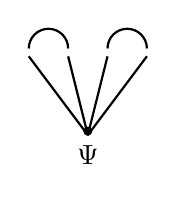
\begin{tikzpicture}[scale=.5, baseline=4mm]
      % node
      \draw[fill=black] (1.5, .1) circle (1mm);
      % lines
      \draw[thick] (1.5, 0) node[anchor=north] {$\Psi$} -- (0, 2);
      \draw[thick] (1.5, 0) -- (1, 2);
      \draw[thick] (1.5, 0) -- (2, 2);
      \draw[thick] (1.5, 0) -- (3, 2);
      % pairings
      \draw[thick] (0, 2.2) arc (180:0:.5);
      \draw[thick] (2, 2.2) arc (180:0:.5);
    \end{tikzpicture}
    +
    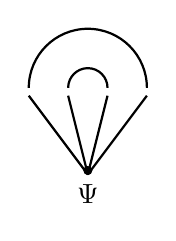
\begin{tikzpicture}[scale=.5, baseline=4mm]
      % node
      \draw[fill=black] (1.5, .1) circle (1mm);
      % lines
      \draw[thick] (1.5, 0) node[anchor=north] {$\Psi$} -- (0, 2);
      \draw[thick] (1.5, 0) -- (1, 2);
      \draw[thick] (1.5, 0) -- (2, 2);
      \draw[thick] (1.5, 0) -- (3, 2);
      % pairings
      \draw[thick] (0, 2.2) arc (180:0:1.5);
      \draw[thick] (1, 2.2) arc (180:0:.5);
    \end{tikzpicture}
    +
    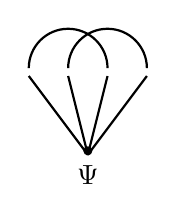
\begin{tikzpicture}[scale=.5, baseline=4mm]
      % node
      \draw[fill=black] (1.5, .1) circle (1mm);
      % lines
      \draw[thick] (1.5, 0) node[anchor=north] {$\Psi$} -- (0, 2);
      \draw[thick] (1.5, 0) -- (1, 2);
      \draw[thick] (1.5, 0) -- (2, 2);
      \draw[thick] (1.5, 0) -- (3, 2);
      % pairings
      \draw[thick] (0, 2.2) arc (180:0:1);
      \draw[thick] (1, 2.2) arc (180:0:1);
    \end{tikzpicture}
    = 3
    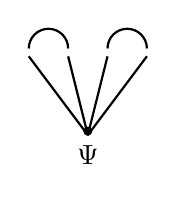
\begin{tikzpicture}[scale=.5, baseline=4mm]
      % node
      \draw[fill=black] (1.5, .1) circle (1mm);
      % lines
      \draw[thick] (1.5, 0) node[anchor=north] {$\Psi$} -- (0, 2);
      \draw[thick] (1.5, 0) -- (1, 2);
      \draw[thick] (1.5, 0) -- (2, 2);
      \draw[thick] (1.5, 0) -- (3, 2);
      % pairings
      \draw[thick] (0, 2.2) arc (180:0:.5);
      \draw[thick] (2, 2.2) arc (180:0:.5);
    \end{tikzpicture}
  \end{equation*}
\end{example}

In general, on $ \avg{ \Psi_1 \otimes \dots \otimes \Psi_r }$ there exists an action of
\begin{equation*}
  S_{d_1} \times \dots \times S_{d_r}
\end{equation*}
therefore we can write
\begin{equation*}
  \bigavg{\frac{1}{d_1!} \Psi_1 \otimes \dots \otimes \frac{1}{d_r!} \Psi_r}
  = \sum_{[\sigma]} \frac{1}{\bigl| \Stab_{[\sigma]} \bigr|}
  (Q^{-1})^{\otimes m} \circ \sigma \circ (\Psi_1 \otimes \dots \otimes \Psi_r)
\end{equation*}
where
\begin{equation*}
  [\sigma] \in \lbigslant{\bigl( \prod_{a = 1}^r S_{d_a} \bigr)}{\text{Matchings}_{2m}}.
\end{equation*}

\begin{example}
  Employing the previous formula we see that
  \begin{equation*}
    \bigavg{\frac{1}{4!} \Psi} = \frac{1}{\bigl| \Stab_{[\sigma]} \bigr|}
    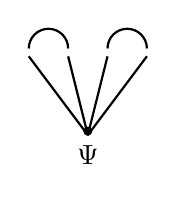
\begin{tikzpicture}[scale=.5, baseline=4mm]
      % node
      \draw[fill=black] (1.5, .1) circle (1mm);
      % lines
      \draw[thick] (1.5, 0) node[anchor=north] {$\Psi$} -- (0, 2);
      \draw[thick] (1.5, 0) -- (1, 2);
      \draw[thick] (1.5, 0) -- (2, 2);
      \draw[thick] (1.5, 0) -- (3, 2);
      % pairings
      \draw[thick] (0, 2.2) arc (180:0:.5);
      \draw[thick] (2, 2.2) arc (180:0:.5);
    \end{tikzpicture}
    = \frac{1}{8} \sum_{i, j, k, l} \Psi_{ijkl} (Q^{-1})_{ik} (Q^{-1})_{jl}.
  \end{equation*}
\end{example}

\begin{example}
  Let $\Psi_1, \Psi_2 \in \Sym^3 V^\vee$. We can verify the previous formula by explicitly computing
  \begin{align*}
    \avg{\Psi_1 \Psi_2}
    &=
    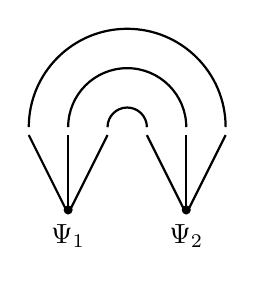
\begin{tikzpicture}[scale=.5, baseline=4mm]
      % nodes
      \draw[fill=black] (1, .1) circle (1mm);
      \draw[fill=black] (4, .1) circle (1mm);
      % lines
      \draw[thick] (1, 0) node[anchor=north] {$\Psi_1$} -- (0, 2);
      \draw[thick] (1, 0) -- (1, 2);
      \draw[thick] (1, 0) -- (2, 2);
      \draw[thick] (4, 0) node[anchor=north] {$\Psi_2$} -- (3, 2);
      \draw[thick] (4, 0) -- (4, 2);
      \draw[thick] (4, 0) -- (5, 2);
      % pairings
      \draw[thick] (0, 2.2) arc (180:0:2.5);
      \draw[thick] (1, 2.2) arc (180:0:1.5);
      \draw[thick] (2, 2.2) arc (180:0:.5);
    \end{tikzpicture}
    + 5 \text{ terms} \\
    &\quad+
    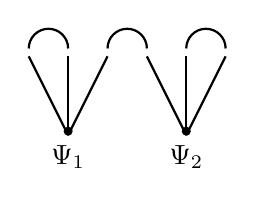
\begin{tikzpicture}[scale=.5, baseline=4mm]
      % nodes
      \draw[fill=black] (1, .1) circle (1mm);
      \draw[fill=black] (4, .1) circle (1mm);
      % lines
      \draw[thick] (1, 0) node[anchor=north] {$\Psi_1$} -- (0, 2);
      \draw[thick] (1, 0) -- (1, 2);
      \draw[thick] (1, 0) -- (2, 2);
      \draw[thick] (4, 0) node[anchor=north] {$\Psi_2$} -- (3, 2);
      \draw[thick] (4, 0) -- (4, 2);
      \draw[thick] (4, 0) -- (5, 2);
      % pairings
      \draw[thick] (0, 2.2) arc (180:0:.5);
      \draw[thick] (2, 2.2) arc (180:0:.5);
      \draw[thick] (4, 2.2) arc (180:0:.5);
    \end{tikzpicture}
    + 9 \text{ terms} \\
    &= 6
    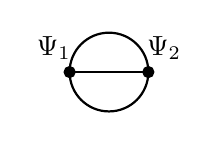
\begin{tikzpicture}[baseline=-1mm]
      % lines
      \draw[thick] (0, 0) node at (-0.2, 0.3) {$\Psi_1$} -- (1, 0) node at (1.2, 0.3) {$\Psi_2$};
      \draw[thick] (0, 0) arc (180:0:.5);
      \draw[thick] (0, 0) arc (-180:0:.5);
      % nodes
      \draw[fill=black] (0, 0) circle (2pt);
      \draw[fill=black] (1, 0) circle (2pt);
    \end{tikzpicture}
    + 9 \ \
    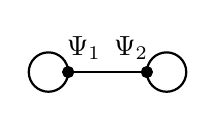
\begin{tikzpicture}[baseline=-1mm]
      % lines
      \draw[thick] (0, 0) node at (0.2, 0.3) {$\Psi_1$} -- (1, 0) node at (0.8, .3) {$\Psi_2$};
      \draw[thick] (-.25, 0) circle (2.5mm);
      \draw[thick] (1.25, 0) circle (2.5mm);
      % nodes
      \draw[fill=black] (0, 0) circle (2pt);
      \draw[fill=black] (1, 0) circle (2pt);
    \end{tikzpicture} \\
    &= \frac{3!3!}{3!}
    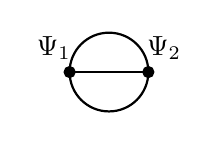
\begin{tikzpicture}[baseline=-1mm]
      % lines
      \draw[thick] (0, 0) node at (-0.2, 0.3) {$\Psi_1$} -- (1, 0) node at (1.2, 0.3) {$\Psi_2$};
      \draw[thick] (0, 0) arc (180:0:.5);
      \draw[thick] (0, 0) arc (-180:0:.5);
      % nodes
      \draw[fill=black] (0, 0) circle (2pt);
      \draw[fill=black] (1, 0) circle (2pt);
    \end{tikzpicture}
    + \frac{3! 3!}{4} \ \
    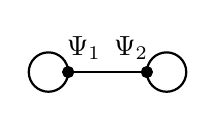
\begin{tikzpicture}[baseline=-1mm]
      % lines
      \draw[thick] (0, 0) node at (0.2, 0.3) {$\Psi_1$} -- (1, 0) node at (0.8, .3) {$\Psi_2$};
      \draw[thick] (-.25, 0) circle (2.5mm);
      \draw[thick] (1.25, 0) circle (2.5mm);
      % nodes
      \draw[fill=black] (0, 0) circle (2pt);
      \draw[fill=black] (1, 0) circle (2pt);
    \end{tikzpicture}.
  \end{align*}
\end{example}

\begin{example}
  The example $\Psi \in \Sym^3 V^\vee$ exhibits more symmetry. As before, we have
  \begin{equation*}
    \avg{\Psi \otimes \Psi}
    = 6
    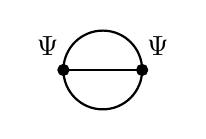
\begin{tikzpicture}[baseline=-1mm]
      % lines
      \draw[thick] (0, 0) node at (-0.2, 0.3) {$\Psi$} -- (1, 0) node at (1.2, 0.3) {$\Psi$};
      \draw[thick] (0, 0) arc (180:0:.5);
      \draw[thick] (0, 0) arc (-180:0:.5);
      % nodes
      \draw[fill=black] (0, 0) circle (2pt);
      \draw[fill=black] (1, 0) circle (2pt);
    \end{tikzpicture}
    + 9 \ \
    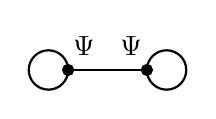
\begin{tikzpicture}[baseline=-1mm]
      % lines
      \draw[thick] (0, 0) node at (0.2, 0.3) {$\Psi$} -- (1, 0) node at (0.8, .3) {$\Psi$};
      \draw[thick] (-.25, 0) circle (2.5mm);
      \draw[thick] (1.25, 0) circle (2.5mm);
      % nodes
      \draw[fill=black] (0, 0) circle (2pt);
      \draw[fill=black] (1, 0) circle (2pt);
    \end{tikzpicture}.
  \end{equation*}
  In this case, there exists an action of $(S_3 \times S_3) \ltimes S_2$ therefore
  \begin{equation*}
    \avg{\Psi \otimes \Psi}
    = \frac{3! 3! 2}{\underbrace{3! 2}_{| \Aut \Lambda |}}
    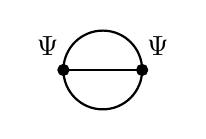
\begin{tikzpicture}[baseline=-1mm]
      % lines
      \draw[thick] (0, 0) node at (-0.2, 0.3) {$\Psi$} -- (1, 0) node at (1.2, 0.3) {$\Psi$};
      \draw[thick] (0, 0) arc (180:0:.5);
      \draw[thick] (0, 0) arc (-180:0:.5);
      % nodes
      \draw[fill=black] (0, 0) circle (2pt);
      \draw[fill=black] (1, 0) circle (2pt);
    \end{tikzpicture}
    + \frac{3! 3! 2}{\underbrace{8}_{|\Aut \Gamma|}} \ \
    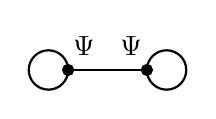
\begin{tikzpicture}[baseline=-1mm]
      % lines
      \draw[thick] (0, 0) node at (0.2, 0.3) {$\Psi$} -- (1, 0) node at (0.8, .3) {$\Psi$};
      \draw[thick] (-.25, 0) circle (2.5mm);
      \draw[thick] (1.25, 0) circle (2.5mm);
      % nodes
      \draw[fill=black] (0, 0) circle (2pt);
      \draw[fill=black] (1, 0) circle (2pt);
    \end{tikzpicture}
  \end{equation*}
  where we identify the denominators with number of automorphisms of the respective graph.
\end{example}

Denote by $\mathsf{Graphs}_{v_0, \dots, v_D}$ the graphs with $v_d$ vertices of valency $0 \leq d \leq D$, where $2m = |HE| = \sum_{d = 0}^D d {v_d}$. There exists a group action
\begin{equation*}
  \prod_{d = 0}^D (S_d)^{v_d} \ltimes S_{v_d} \acts \text{Matchings}_{2m}
\end{equation*}
with what corresponds to graph isomorphisms.
